\documentclass[pdftex,12pt,letter]{article}

\usepackage{verbatim}
\usepackage{graphicx}
\usepackage{placeins}
\usepackage{enumerate}
\usepackage{hyperref}
\makeatletter
  \renewcommand\@seccntformat[1]{\csname the#1\endcsname.\quad}
\makeatother
\newcommand{\HRule}{\rule{\linewidth}{0.5mm}}
\begin{document}

\begin{titlepage}
\begin{flushright}
\HRule \\
{\huge \bfseries Case Scheduler\\[4cm]}
{\large Prepared by\\Jason Kuster, Stuart Long, and Nathan McKinley\\[1cm]
December 7, 2012}
\end{flushright}
\end{titlepage}
\tableofcontents{}
\newpage
\section{Introduction Overview}
Currently, there only exist functional but not particularly elegant ways for students to visualize their class schedules. For our project, we want to make a better Case Scheduler, one which works fast and is easy for students to use.\\

\noindent When making a class schedule, it is very helpful to be able to see what your schedule looks like. The two systems currently available, SIS and scheduler.case.edu do an unsatisfactory job of displaying the schedule. The problem with SIS is that it's exceedingly slow and inefficient for course planning, and is much more suited to only doing course enrollment. The problem with scheduler.case.edu is that not only is it slow to open and do anything, but it is impossible to print without using the Print Screen function on your computer, exporting it to an image, and printing that image. In addition, there are many expansions which could be made to functionality, such as easy sharing of schedules and planning your schedule with friends. What we plan to do is to duplicate the functionality of the current Case Scheduler, while completely rewriting the user interface and backend code to allow for a better user experience.\\

\noindent We will be using two technologies to implement this scheduler. First, we will be using Python and the Django framework for programming our web application. Second, we will be using MySQL for our database.
\section{Application Requirements Specifications}
\begin{enumerate}[1.]
\item The system will maintain a per-user list of courses.\\\\
This is the main focus of our project. Our object is to create a place to which students are able to come and put in and plan their schedule. In order for this to happen, we must maintain per-user lists of courses. These lists of courses will be maintained for four years, after which point they will be discarded. We will allow for creation of lists for the current semester, as well as the next semester once the data is available from the Student Information System.
\item The system will allow the user to search the catalog for courses.\\\\
In order to create their lists of courses, users must be able to find the courses they wish to take. Our system will support searching by course name and will match queries based on course name, description, and instructor. The search results will be displayed in a convenient list view, with the differences clearly marked (course name, meeting time, instructor, etc). The current Case Scheduler view is shown below.\\
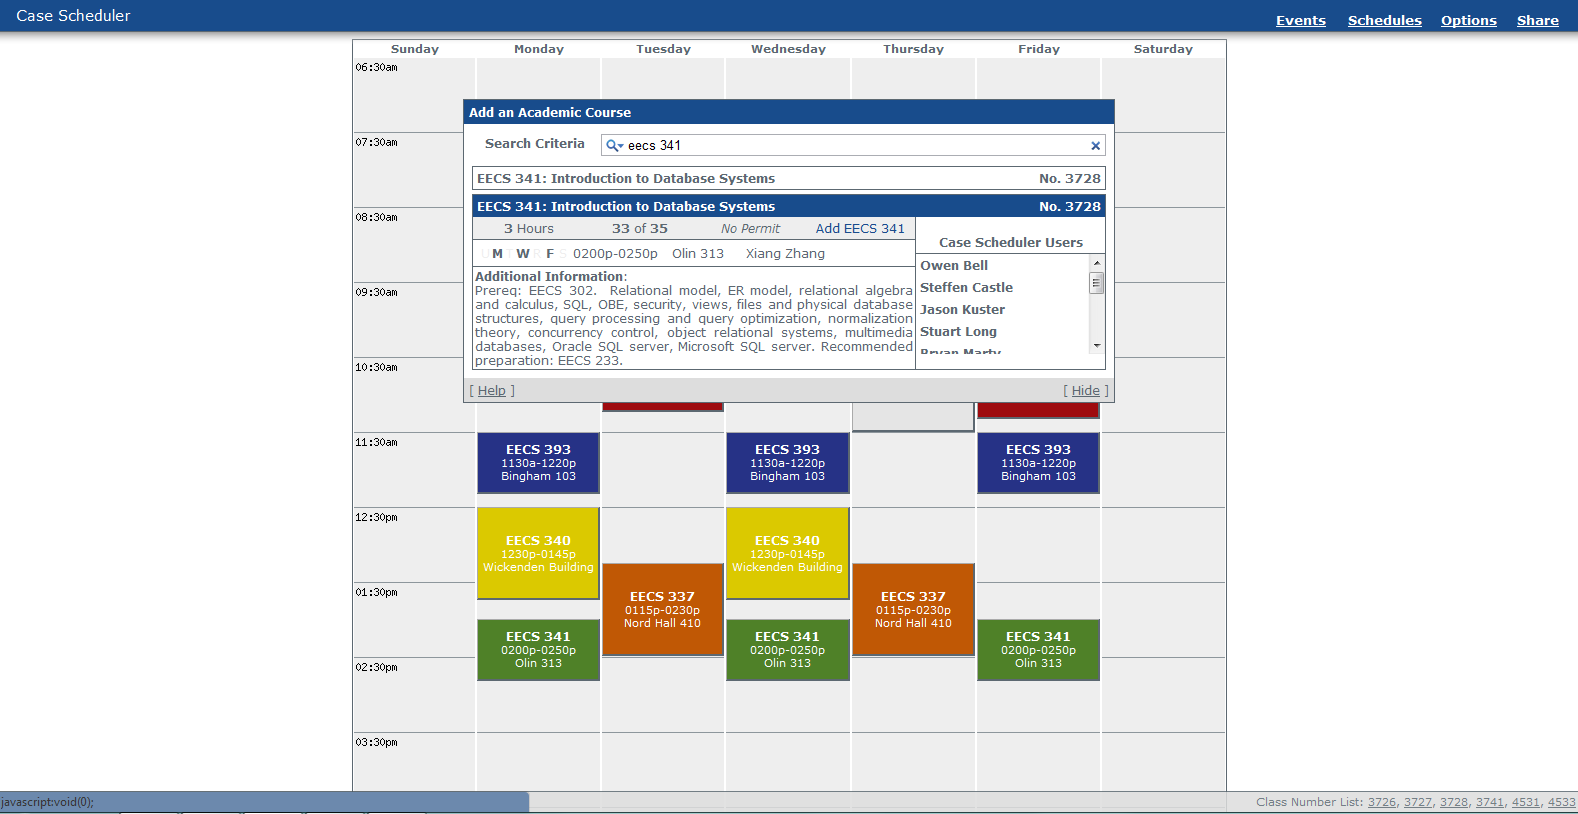
\includegraphics[width=130mm]{add_course.png}
\item The system will allow courses to be added to users' active schedule.\\\\
Once found, a course must be able to be added to a user's currently active schedule. It should stay there until removed either by them or by the system. The functionality of this will be very similar to the functionality of the current Case Scheduler, as shown in the above graphic, but will have a reworked user interface designed by our team.
\item The system should support removing a course from a particular schedule.\\\\
As a user's courses can change during the planning stages or during drop/add, users should be able to remove courses which they have added from their lists.
\item The system will display course information on a weekly calendar-formatted schedule, including course name, times, instructor, and location.\\\\
This format seems to be the easiest and most convenient to view, and gives users a quick and easy-to-use overview of their courses for the week. In the future, other layouts such as a list-type view, day-by-day view, and monthly view. Our implementation of the weekly view will look similar to the below graphic, although with a rewritten user interface backend.\\
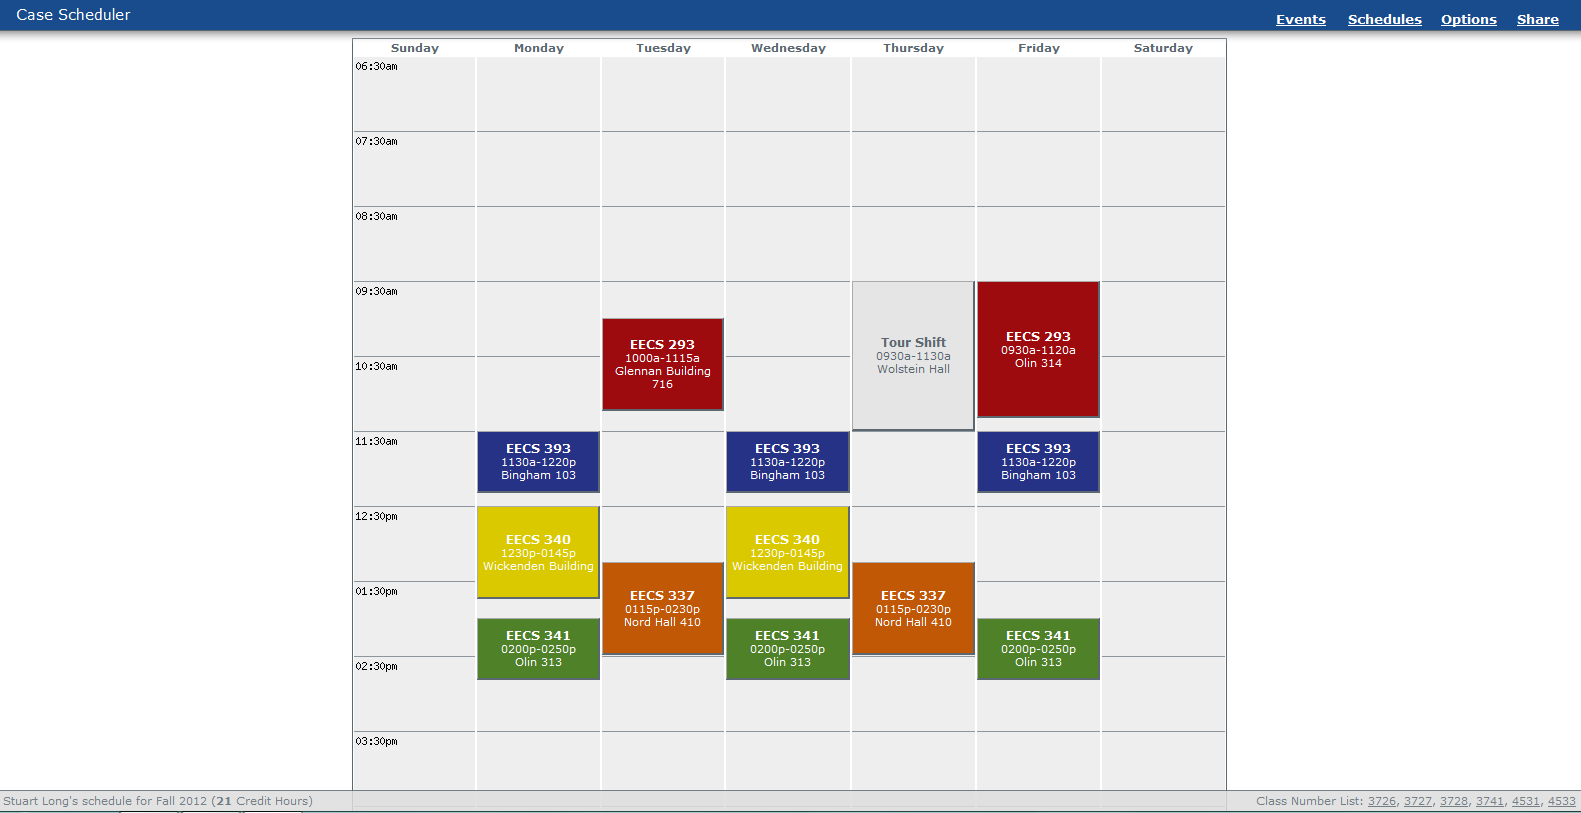
\includegraphics[width=130mm]{main_schedule.png}
\item The system should display itself in a manner which facilitates printing.\\\\
The current system makes it exceedingly difficult to print one's schedule. We are making sure that by design our system will be formatted for printing without users having to do anything.
\item The system should maintain users' lists across SIS updates.\\\\
As the list of courses is subject to change as courses are added or removed in SIS, we will make sure that our application remains robust across these changes and that when responding to changes in the schedule of classes xml file, we do not inadvertently break anyone's schedule.
\item Clicking on courses will bring up more detailed course information.\\\\
As there is a wealth of information about the courses in SIS, we plan to make that data consumable by our users by adding a detail page to each course. This detail page will include such items as classroom, teacher, and meeting times, among others.
\item Under reasonable load, the system should have loading times of less than one second.\\\\
At the current time, scheduler.case.edu can take upwards of 15 seconds to properly aggregate and display all of a user's classes. This frustrates users and is a design flaw which should be easily remediable. Our system will have much faster response times, ensuring greater user satisfaction and a more usable product.
\item The system will allow users to change their current working semester, and will maintain schedules up to 4 years in the past.\\\\
This is necessary in order to allow users to plan a next semester while having a schedule for their current semester. The second SIS data is available, we will make it available to the students and allow them to start planning their next semester. In addition, the ability to go and see what courses they have taken in previous semesters provides value because students will no longer have to do the time-consuming process of using SIS.
\item The system supports the creation of custom events.\\\\
In order to be a one-stop schedule manager, as well as to remain more feature-complete than the current case scheduler, we will be adding support for custom events such as TA sessions, jobs, and other user-defined events. These custom events will have all of the behavior of courses, but will be visible only to their creator, i.e they will not appear in searches. The add dialog will look similar to below.\\
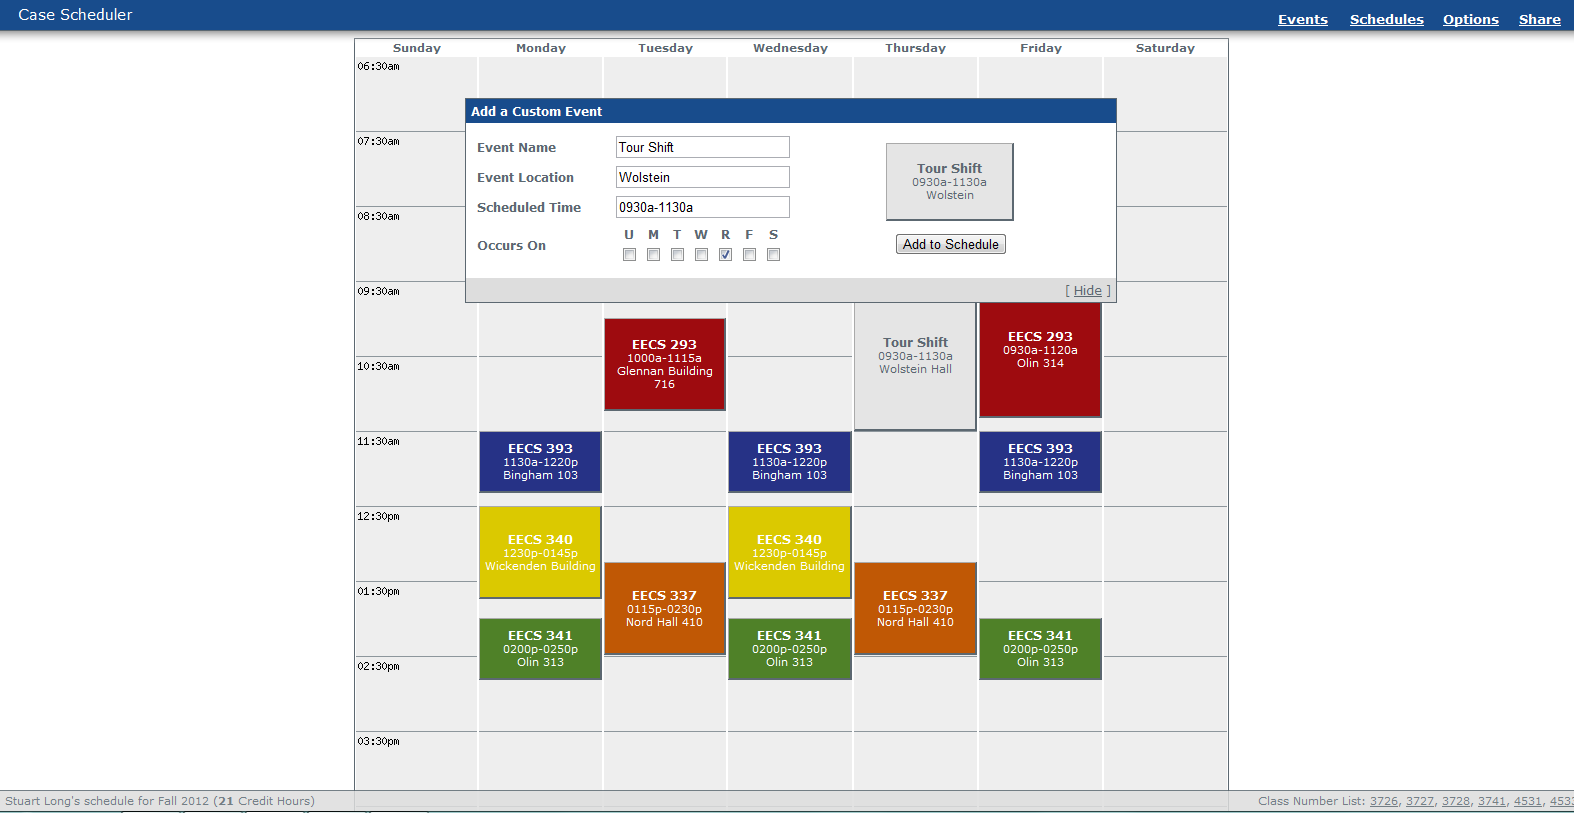
\includegraphics[width=130mm]{add_event.png}
\end{enumerate}
\section{Database Requirements Specifications}
\subsection{Objects and Relationships}
\begin{enumerate}[1.]
\item Course Offering: The database will have an instance of course offering for each course offered by CWRU. Every course offering is-a course, which is described below. This entity it important to our application because a course offering is the typical item that a user will actually had to his or her schedule. A course offering will have at least the following attributes: offering id, term, subject, status, dates, days/times, room, total capacity, current enrollment, and description.\\\\  In explanation, the "component" attribute represents the type of the course, whether it's a lecture, recitation, or similar. The "status" attribute represents whether the course is  open, closed, or other, which is important for a user to know when scheduling for a certain course. "Current Enrollment" signifies how many other students are registered for the course offering. "Description" is a paragraph explanation of the course provided by the department or professor, also important info for a user browsing through various courses.
\item Course: every course offering is-a course. A course entity is useful to have for this application because it will allows the application to more easily display all of the course offering for a selected course. The course entity will have the following attributes: title, catalog number, component, units (max), and label. In explanation, the "label" attribute corresponds to a short combination of the of the subject, catalog number, and title. The catalog number corresponds to the course number within that courses department (e.g. 314 for EECS 341). Courses will also have prerequisite as specified by the Has\_Prerequisite relationship, detailed below.
\item Has\_Prerequisite Relationship: This relationship involves only Course entities. Any one course may have multiple prerequisites and may be a prerequisite for multiple courses. This relationship will allow the application to easily display and direct users to what prerequisites a given course may have.
\item User: Every user will log onto our application with their case id and password (using the single sign on service as provided by CWRU). This process allows us to keep an object representation of each user. This application doesn't need much information about each user, so it will just keep track of the user's case id and last login date. We keep track of their login date so we can safely delete a user and any relationships that user participated in after the user has not logged in for four years.
\item Instructor: Our application will allows users to find basic information about CWRU instructors, such as office location, office hours, and contact information. To adequately display this information, the instructor object will have at least the following attributes: instructor ID, office location, office hours, phone number, and email.
\item Teaches Relationship: Every course offering will be taught by an instance of instructor, and this relation models that, simply by storing the id's for the course offering and the instructor that teaches it. We assume a course offering is not taught by more than one instructor, an assumption that is sufficient for a scheduling application.
\item Enrolled-in Relationship: Multiple students can take multiple different courses, and courses can have many students enrolled in it, up to that courses capacity. This relationship is fairly simple in that it just keeps track of a student and a course that student is enrolled in. However, it is also an extremely important relationship because it allows us to populate a students schedule.
\item Custom Event: Like the current Case Scheduler, our application will allow users to add their own recurring custom events to the schedule. A good example might be an extra-curricular actives such as band rehearsals or sport practices. As such, the databases needs a separate entity to store these events. This entity will have the following attributes: days/times, location, title, semester, and description. This entity will be a weak entity and each custom event will be connected to a single user through the Has relationship.
\item Has Relationship: The Has relationship, again, connects users to the custom events they have created. This relationship is a one-to-many relationship, so a user may have many custom events, and it requires full participation on the part of the custom event entities.
\end{enumerate}
\subsection{Queries and Transactions}
\begin{enumerate}[1.]
\item Get\_List:  Since the application is centered around displaying a graphical representation of a list of courses, we will need to retrieve the list of courses associated with the current user.  Since we will not be storing this list in cookies, we will need to retrieve it from the database every time we seek to display it.  This will be required approximately once per page-view.  This will require as input the user ID (Case ID), and produce as output a list of course ids.
\item Lookup\_Course:  Since the application will need to display information about each course in the list of courses, we will need to retrieve this information.  This information will include things like course title, course description, instructor, course time, and course location.  Since most lists will contain more than one course, we will need to perform this query more than one time per page view.  This query will require as input a course ID, and will return several columns which will be used to build the calendar.
\item Add\_Course:  Since the application requires that a user build a list of courses, the user will be need to be able to build the list of courses by adding to it.  We will add courses to the user lists using this transaction.  This transaction will take as input the user ID and a course ID and will add the course ID to the list of courses for the user in question.  It will not return anything.  This will be done much less than once per page view, since the average user will need to view their courses more than once, but will only need to add them one time each.
\item Remove\_Course:  The opposite of Add\_Course, sometimes users will need to remove courses that they've already added.  This will happen even less often than Add\_Course, because most users will only add courses that they plan to view in the future.  Most users do not drop courses, and so most users will only need to add courses.  This will happen far less than once per page view.  This transaction will take as input the User ID and Course ID, and will delete the row from the table pairing users and courses, and will not return anything.
\item Lookup\_Instructor:  One feature that users might desire is the ability to lookup all courses that a particular instructor is teaching.  This means that we will want to index the courses table by instructor as well as by course ID.  This query will be used much less frequently than the other queries and transactions because the primary feature of the application is display of a calendar, not viewing the courses taught by a particular instructor.  This transaction will take as input the instructor name, and will return a list of course IDs taught by that instructor.
\item Create\_Event: Users will be allowed to create their own custom events to add to any schedule they desire. The application will use the event's semester attribute to determine which schedule to add the event to.
\end{enumerate}
\subsection{Actions and Events}
\begin{enumerate}[1.]
\item This application will display users' schedules based on the currently selected semester, with the default semester being the current semester at the time of the user login. The application will have a drop down list or similar form that will allow users' to select any other schedule in which the user has a course. As can be seen above, the database does not have an actual "schedule" object. To craft various semester schedules, the course offering relations will just be queried for term and the user's schedules will be constructed off of that. All of a user's schedules will be stored until that user is deleted, see \textit{Integrity Constraints} for user deletion policies.
\item An event that will happen every time the application is used by any user is a user login. To use this application a user must have a CWRU ID and password, and will log in with the CWRU Single Sign-On Service. By logging in, the application will be able to identify the user and load all of that user's schedules.
\end{enumerate}
\subsection{Integrity Constraints}
\begin{enumerate}
\item Users must be enrolled in at least one course offering. If, for some reason, a user is no longer enrolled in any course offering, then that user is removed from the database. If the user wants to use an application after being deleted, than a new "user" object for that user will be created upon log-in, as if that user was a first time user.
\item This application may have to handle up to all CWRU community members and several schedules per user. In order to maintain a flexible ceiling on the database, users that have been inactive for more than four years. If a user is removed and one of the course offerings that that user was enrolled in no longer has any users enrolled in it, then that course offering is deleted as well.
\item If, at any time, a course offering has no users enrolled in it, and the current semester is after the semester that course offering took place in, then that course offering will be removed.
\item Instructors are allowed to not teach a course offering at any given time. However, if an instructor continuously does not teach a course for five years, then that instructor is removed.
\item Every custom event must be involved in a Has relationship with some user.
\item Every course offering must satisfy the is-a course relationship.
\end{enumerate}
\section{ER Diagram}
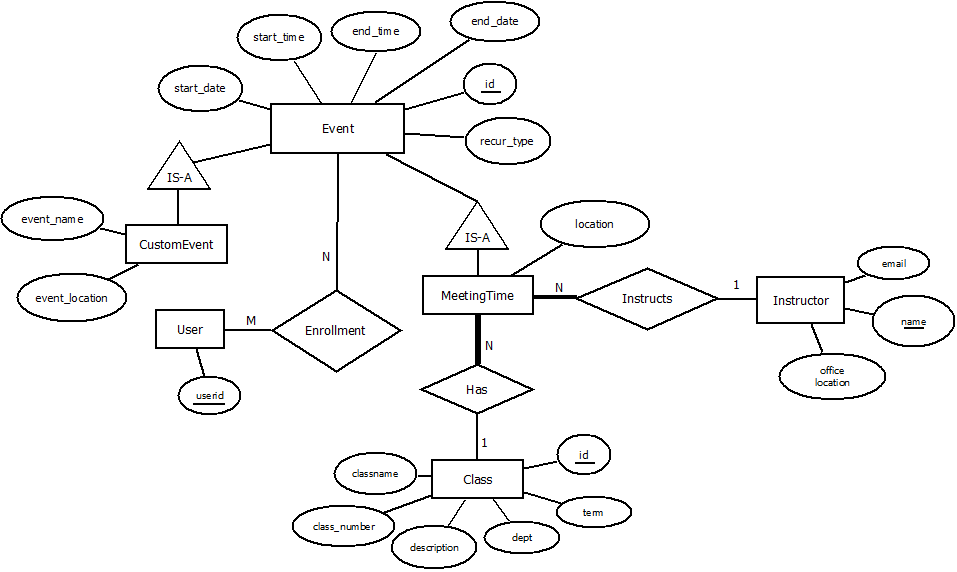
\includegraphics[width=120mm]{ERDiagram.png}
\FloatBarrier
\pagebreak
\section{Relational Model}
\begin{verbatim} 
BEGIN;
CREATE TABLE `course_scheduler_class` (
    `id` integer AUTO_INCREMENT NOT NULL PRIMARY KEY,
    `class_number` integer NOT NULL,
    `dept` varchar(10) NOT NULL,
    `classname` varchar(350) NOT NULL,
    `description` varchar(4096) NOT NULL,
    `term` varchar(30) NOT NULL
)
;
CREATE TABLE `course_scheduler_event` (
    `id` integer AUTO_INCREMENT NOT NULL PRIMARY KEY,
    `start_time` time NOT NULL,
    `end_time` time NOT NULL,
    `start_date` date NOT NULL,
    `end_date` date NOT NULL,
    `recur_type` varchar(12) NOT NULL
)
;
CREATE TABLE `course_scheduler_customevent` (
    `event_ptr_id` integer NOT NULL PRIMARY KEY,
    `event_name` varchar(120) NOT NULL,
    `location` varchar(50) NOT NULL
)
;
ALTER TABLE `course_scheduler_customevent` ADD CONSTRAINT `event_ptr_id_refs_id_4813623e` FOREIGN KEY (`event_ptr_id`) REFERENCES `course_scheduler_event` (`id`);
CREATE TABLE `course_scheduler_meetingtime` (
    `event_ptr_id` integer NOT NULL PRIMARY KEY,
    `meeting_class_id` integer NOT NULL,
    `meeting_location` varchar(50) NOT NULL
)
;
ALTER TABLE `course_scheduler_meetingtime` ADD CONSTRAINT `meeting_class_id_refs_id_8beceb5b` FOREIGN KEY (`meeting_class_id`) REFERENCES `course_scheduler_class` (`id`);
ALTER TABLE `course_scheduler_meetingtime` ADD CONSTRAINT `event_ptr_id_refs_id_98bafe7b` FOREIGN KEY (`event_ptr_id`) REFERENCES `course_scheduler_event` (`id`);
CREATE TABLE `course_scheduler_instructor` (
    `email` varchar(10) NOT NULL,
    `name` varchar(50) NOT NULL PRIMARY KEY,
    `office` varchar(15) NOT NULL
)
;
CREATE TABLE `course_scheduler_instructs` (
    `id` integer AUTO_INCREMENT NOT NULL PRIMARY KEY,
    `instructor_id` varchar(50) NOT NULL,
    `meeting_id` integer NOT NULL
)
;
ALTER TABLE `course_scheduler_instructs` ADD CONSTRAINT `instructor_id_refs_name_d0e02416` FOREIGN KEY (`instructor_id`) REFERENCES `course_scheduler_instructor` (`name`);
ALTER TABLE `course_scheduler_instructs` ADD CONSTRAINT `meeting_id_refs_event_ptr_id_4ac340b8` FOREIGN KEY (`meeting_id`) REFERENCES `course_scheduler_meetingtime` (`event_ptr_id`);
CREATE TABLE `course_scheduler_student` (
    `case_id` varchar(6) NOT NULL PRIMARY KEY
)
;
CREATE TABLE `course_scheduler_enrollment` (
    `id` integer AUTO_INCREMENT NOT NULL PRIMARY KEY,
    `student_id` varchar(6) NOT NULL,
    `event_id` integer NOT NULL
)
;
ALTER TABLE `course_scheduler_enrollment` ADD CONSTRAINT `student_id_refs_case_id_70e0330d` FOREIGN KEY (`student_id`) REFERENCES `course_scheduler_student` (`case_id`);
ALTER TABLE `course_scheduler_enrollment` ADD CONSTRAINT `event_id_refs_id_6200046` FOREIGN KEY (`event_id`) REFERENCES `course_scheduler_event` (`id`);
COMMIT;
\end{verbatim}
\subsection{Justification of Relational Model}
\begin{itemize}
\item User HAS Custom Event (1:N, full participation from Custom Event to Has)
\subitem This relationship is satisfied by two pieces: first, the Custom Event has a key for the id of the user to which it is attached. This satisfies the 1:N part of the relationship. Second, the id is listed as NOT NULL, which enforces the full participation.
\item User Enrolled-In Course Offering (M:N)
\subitem This relationship is satisfied by the inclusion of the Enrolled-In table, which contains a user id and an offering id.
\item Instructor Teaches Course Offering (1:N, full participation from Instructor to Course Offering)
\subitem This relationship is satisfied by two pieces: first, each Course Offering has an Instructor id key corresponding to the instructor who teaches the class. This satisfies the 1:N part of the relationship. The full participation from Course Offering to Teaches is enforced by the NOT NULL on the Instructor ID.
\item Course Offering IS-A Course
\subitem The IS-A relationship here is satisfied by having each Course Offering contain a catalog number, which connects it to a specific instance of a course. It thus becomes an instance of that course.
\item Course Has\_Prerequisite
\subitem The Has\_Prerequisite relationship is satisfied by the inclusion of the Has\_Prerequisite table. It contains two keys, one key for the course in question, and another for the course for which it is a prerequisite. In this way, one course can have multiple prerequisites and can also be a prerequisite for multiple classes.
\end{itemize}
\section{Installing on a DBMS}
We successfully installed mysql on a linux machine that one of our group members owns.  The machine is running Ubuntu, so the installation was a very straightforward process.  We simply ran 'apt-get install mysql-server'.  After that, we needed to create the scheduler database, which was done simply:\\\\
\begin{verbatim}
CREATE DATABASE scheduler;
USE scheduler;
\end{verbatim}

Then it got fairly complicated.  It became apparent (see figure 1) that the syntax we've been using wasn't correct.  In mysql, foreign key constraints need to be declared after the keys themselves; in the SQL we learned, they could be declared at the end of the CREATE TABLE statement.  This correction was necessary throughout the set of table creations.  About halfway through it became clear how the SQL needed to be modified.  We then used DESCRIBE calls to ensure that everything was set up correctly.
\begin{flushleft}
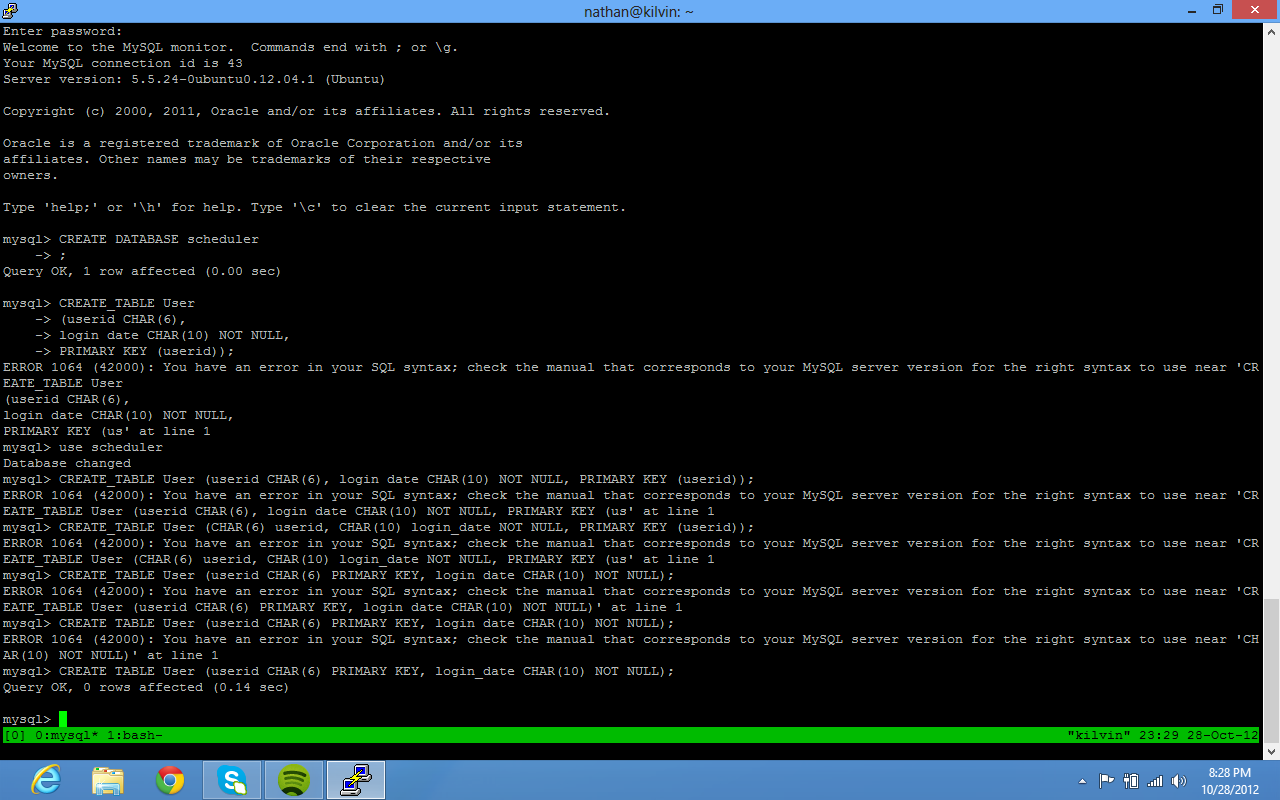
\includegraphics[width=4in]{db1.png}
\FloatBarrier
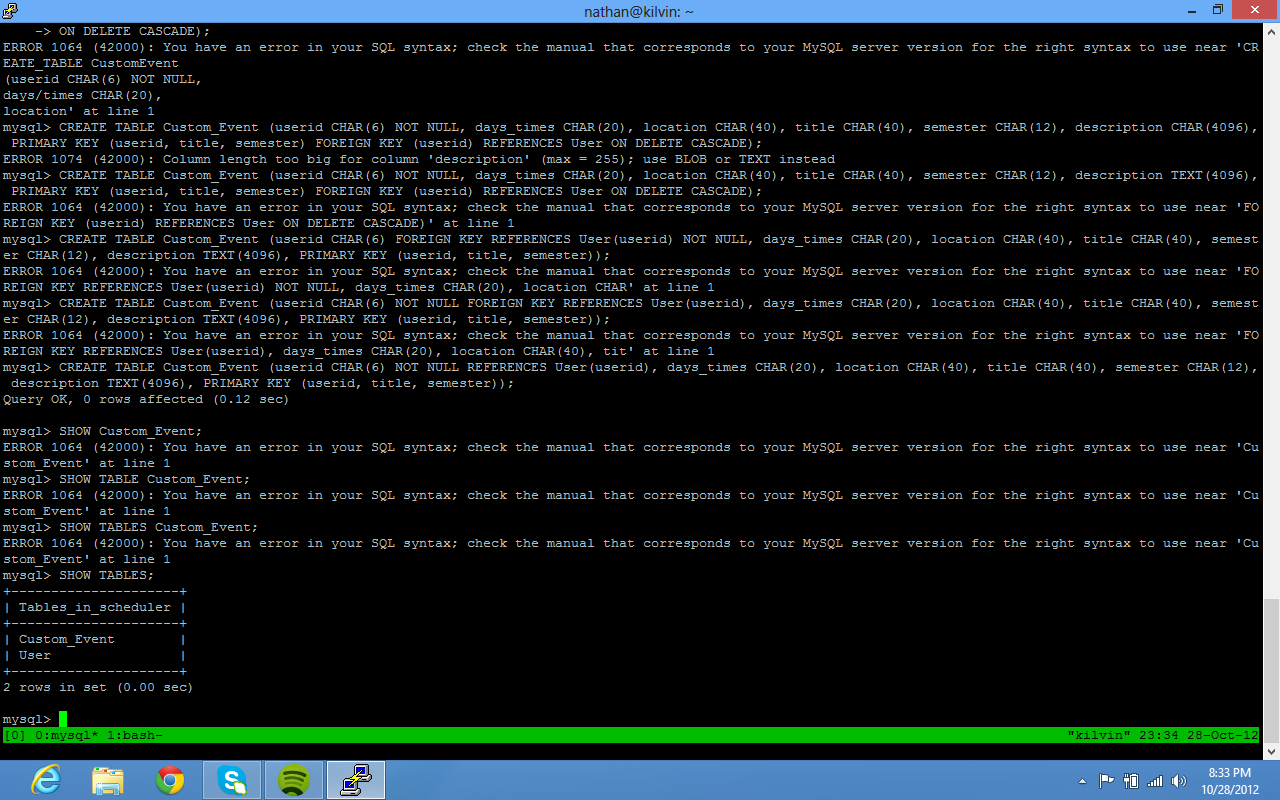
\includegraphics[width=4in]{db2.png}
\FloatBarrier
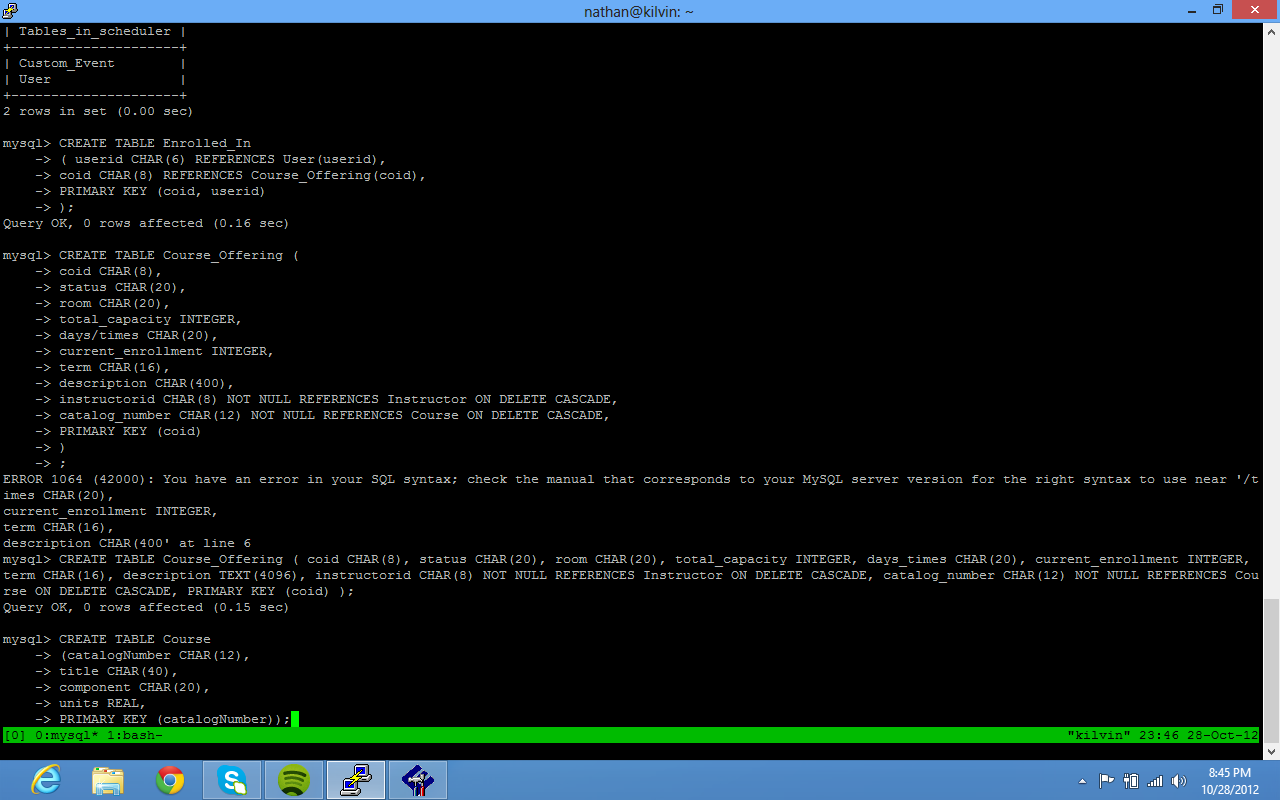
\includegraphics[width=4in]{db3.png}
\FloatBarrier
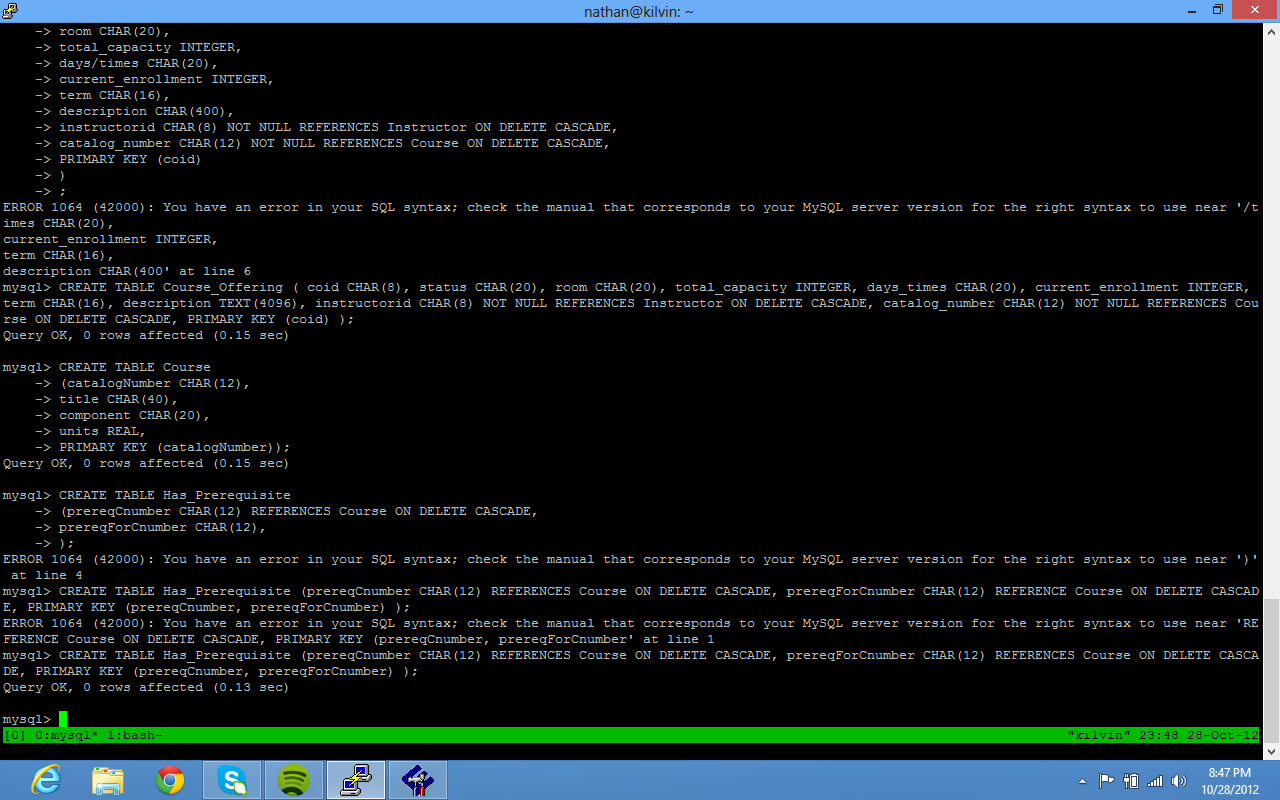
\includegraphics[width=4in]{db4.png}
\FloatBarrier
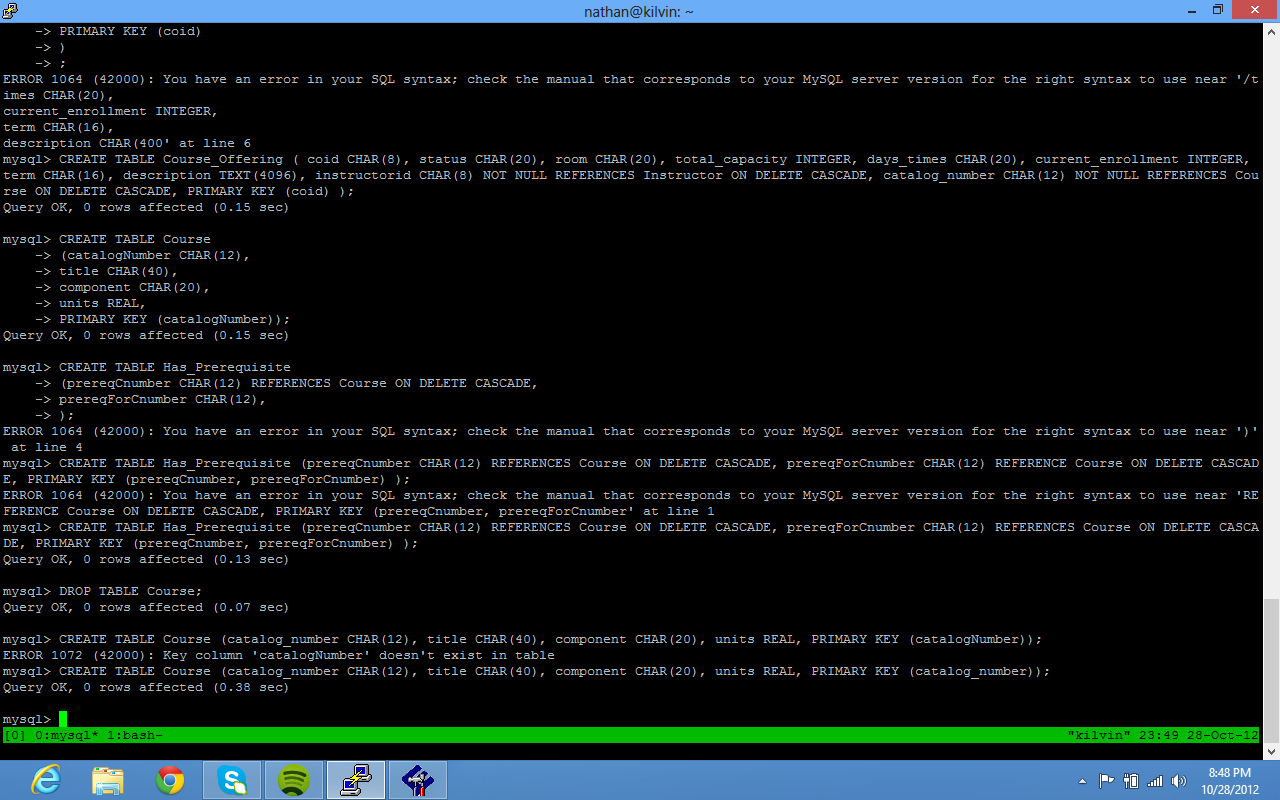
\includegraphics[width=4in]{db5.png}
\FloatBarrier
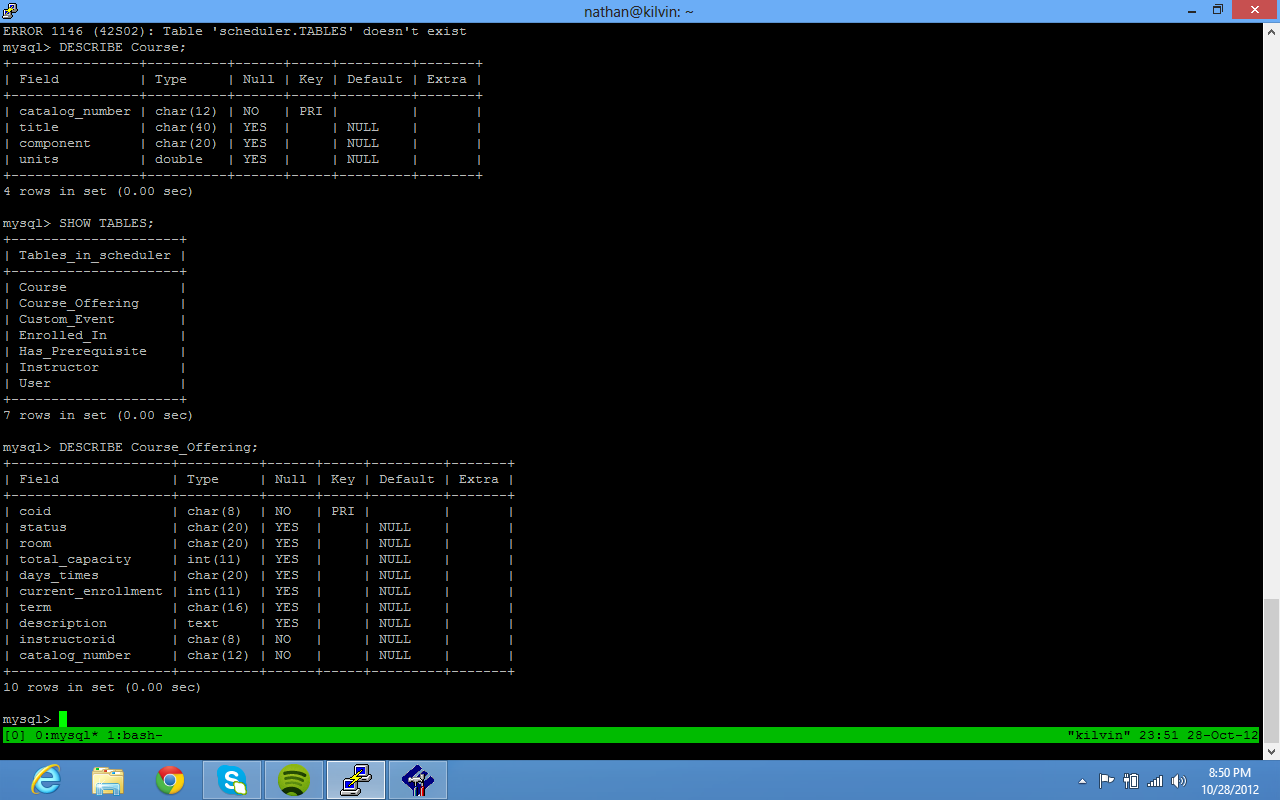
\includegraphics[width=4in]{db6.png}
\FloatBarrier
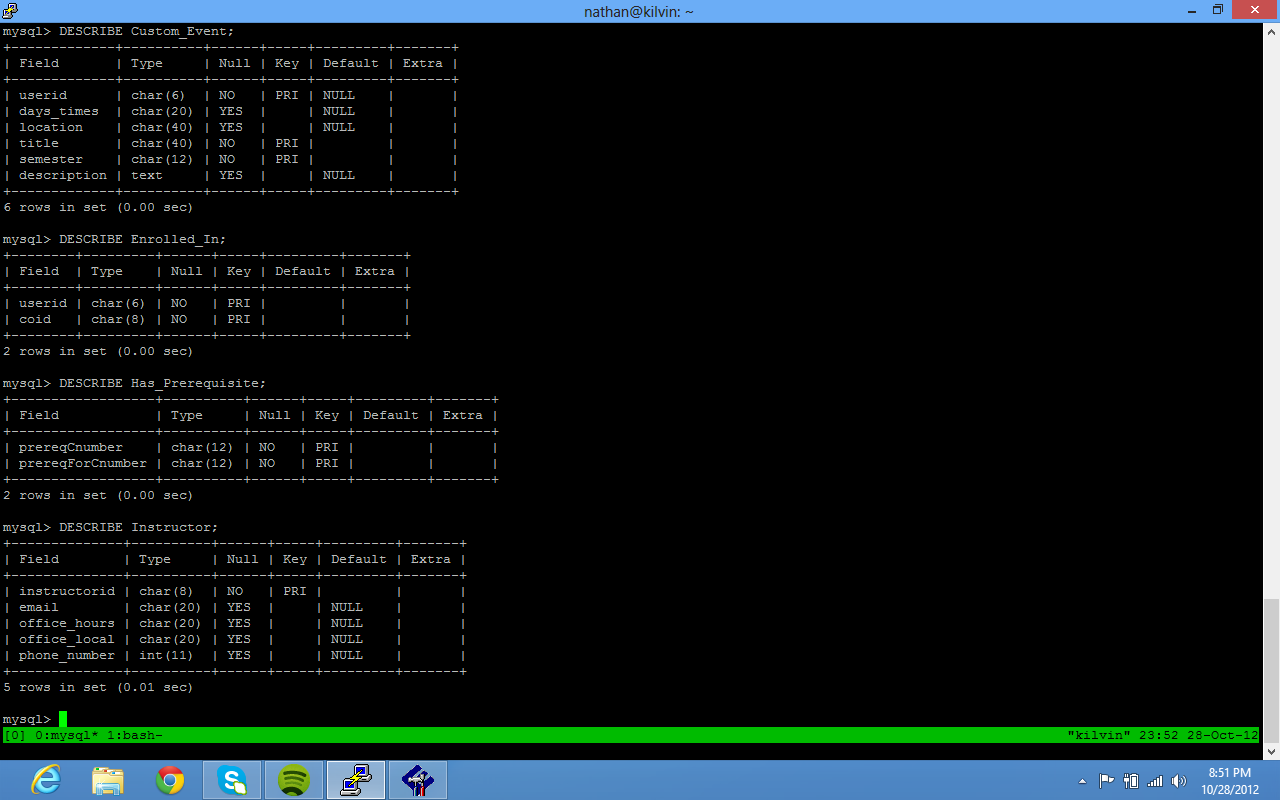
\includegraphics[width=4in]{db7.png}
\FloatBarrier
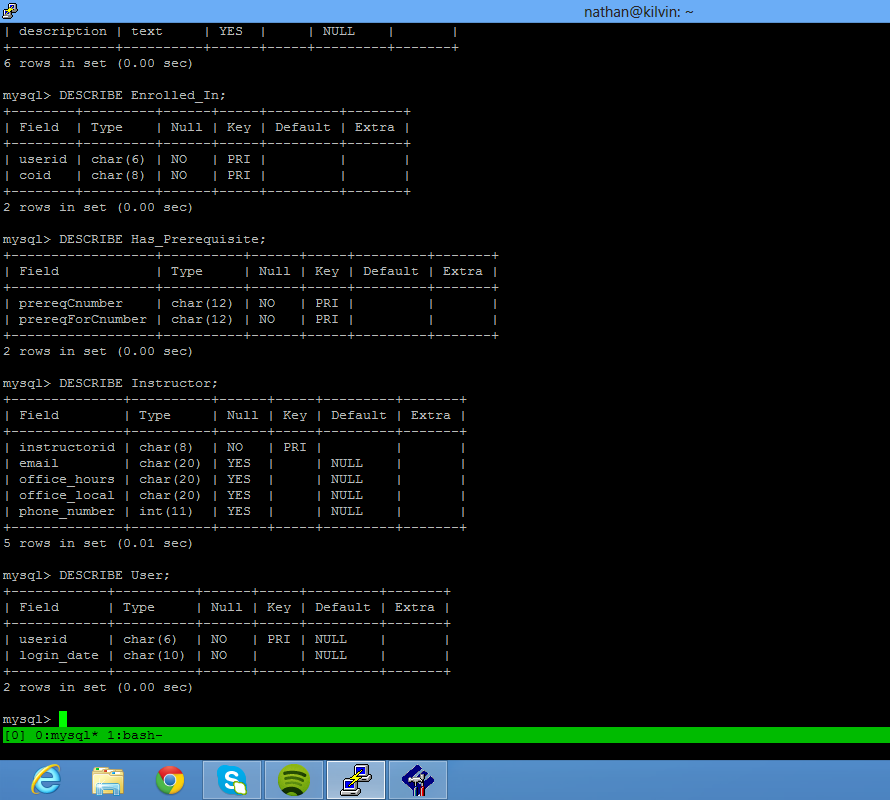
\includegraphics[width=4in]{db8.png}
\FloatBarrier
\end{flushleft}

\section{SQL Queries}
Due to the nature of our application, our queries do not get terribly crazy.
\begin{enumerate}[1.]
\item Query: All instructs tuples whose events have a given dept/number combination.
\begin{enumerate}[i.]
\item RA: 
\item TRC: $\{v^2\vert(\exists i)(\exists m)(\exists c)(\exists)(Instructs(i) \wedge MeetingTime(m) \wedge Class(c) \wedge v[1]=i.instructor \wedge v[2]=i.meeting \wedge i.meeting=m.id \wedge m.meeting\_class = c.pk \wedge c.dept=input\_dept \wedge c.class\_number = input\_number)\}$
\item SQL:
\end{enumerate}
\item Query: All instructs tuples whose events have a dept that contains a passed string
or have a number that contains a passed string or whose names contains a
passed string
\begin{enumerate}[i.]
\item RA:
\item TRC:$\{v^2\vert(\exists i)(\exists m)(\exists c)(\exists)(Instructs(i) \wedge MeetingTime(m) \wedge Class(c) \wedge v[1]=i.instructor \wedge v[2]=i.meeting \wedge i.meeting=m.id \wedge m.meeting\_class = c.pk \wedge (Contains(c.dept, input\_dept) \vee Contains(c.number, input\_number) \vee Contains(c.classname, input\_name)))\}$
\item SQL:
\end{enumerate}
\item Query: All instructs tuples whose meetings are in an enroll relation with a
passed student's id
\begin{enumerate}[i.]
\item RA:
\item TRC: $\{v^2\vert(\exists i)(\exists m)(\exists en)(Instructs(i) \wedge MeetingTime(m) \wedge Enrollment(e) \wedge v[1]=i.instructor \wedge v[2]=i.meeting \wedge i.meeting=m.id \wedge en.student=input\_id \wedge en.event=m.id)\}$
\item SQL:
\end{enumerate}
\item Query: All instructs tuples whose instructor's name matches exactly a passed string
\begin{enumerate}[i.]
\item RA:
\item TRC: $\{v^2\vert(\exists i)(\exists p)(Instructs(i) \wedge Instructor(p) \wedge v[1]=i.instructor \wedge v[2]=i.meeting \wedge i.instructor=p.name \wedge p.name=input\_name\} $
\item SQL:
\end{enumerate}
\item Query: the event with a passed id that is in an enroll relationship with a
student with a passed id
\begin{enumerate}[i.]
\item RA:
\item TRC: $\{v^6 \vert (\exists ev)(\exists en)(Enrollment(en) \wedge Event(ev) \wedge v[1]=ev.start\_time \wedge v[2]=ev.end\_time \wedge v[3]=ev.start\_date \wedge v[4].ev.end\_date \wedge v[5]=ev.recur\_type \wedge v[6]=ev.id \wedge en.event = ev.id \wedge en.student=input\_case\_id \wedge ev.id=\wedge input\_event\_id)\}$
\item SQL:
\end{enumerate}
\end{enumerate}

\section{Integrity Constraints}

Our first and most wide-reaching integrity constraint is that we require all character fields to be non-null, but allow storing of empty values.  This is enforced by our backend.
We have the following less trivial constraints:  the id field of the Class table must be non-null.  We resorted to an id field because our database backend is currently unable to handle multi-column keys, and there is no single column which is a key for a class.  This is enforced by the backend as it's a primary key of the table.  
The id field of Event also must be non-null.  We decided on an id field instead of a multi-column key for the same reason as above.  We made this decision beacuse there are two tables that have the IS-A relation with Event (MeetingTime and CustomEvent), and our database framework implements inheritance by selecting a foreign key to the parent table as the primary key for the child tables.
MeetingTime and CustomEvent have primary keys that must be present in Event.  This is enforced by our database backend.  MeetingTime's meeting\_class attribute must refer to an id that is present in Class.
Instructor has 'name' as a primary key, so names must be unique.
Instructs has an ID which must be unique.  The instructor attribute must refer to a name that is present in the Instructor table.  The meeting attribute must refer to an id which is present in MeetingTime.
The Student table contains only a case\_id and that's the primary key.  The Enrollment table has an id attribute which must be non-null, a foreign key to Student which is the case\_id of the student in question (must be present in Student, enforced by backend), and a foreign key to Event's id (must be present in Event, enforced by backend).\\

We also have one subtler constraint which is not enforced by the backend.  An Event must be either a CustomEvent, a MeetingTime, or neither.  If Event's id is present in both MeetingTime and CustomEvent, if a student enrolls in the Event, it is unclear whether the name associated with the MeetingTime or the CustomEvent should be displayed.  We deal with this by displaying the MeetingTime if it ever happens, but also by creating a new Event for every MeetingTime or CustomEvent.\\

\section{Relational Database Design -- Applying The Dependency Theory}
As we have a relatively straightforward database structure, all of our relations are already in BCNF(and thus 3NF). They are listed below:
\subsection*{Class}
\begin{itemize}
\item c\_id (Primary Key)
\item class\_number
\item dept
\item classname
\item description
\item term
\end{itemize}
c\_id $\rightarrow$ class\_number, dept, classname, description, term (In BCNF since c\_id is a key)
\subsection*{Event}
\begin{itemize}
\item id (Primary Key)
\item start\_time
\item end\_time
\item start\_date
\item end\_date
\item recur\_type
\end{itemize}
id $\rightarrow$ start\_time, end\_time, start\_date, end\_date, recur\_type (In BCNF since id is a key)
\subsection*{CustomEvent}
\begin{itemize}
\item id (Primary Key)
\item event\_name
\item location
\end{itemize}
id $\rightarrow$ event\_name, location (In BCNF since id is a key)
\subsection*{MeetingTime}
\begin{itemize}
\item id
\item meeting\_class
\item meeting\_location
\end{itemize}
id $\rightarrow$ meeting\_class, meeting\_location (In BCNF since id is a key)
\subsection*{Instructor}
\begin{itemize}
\item email
\item name (Primary Key)
\item office
\end{itemize}
name $\rightarrow$ email, office (In BCNF since name is a key)
\subsection*{Instructs}
\begin{itemize}
\item Instructor (Foreign Key $\rightarrow$ Instructor)
\item Meeting (Foreign Key $\rightarrow$ MeetingTime)
\end{itemize}
No Functional Dependencies (In BCNF because no Functional Dependencies)
\subsection*{Student}
\begin{itemize}
\item case\_id (Primary Key)
\end{itemize}
No Functional Dependencies (In BCNF because no Functional Dependencies)
\subsection*{Enrollment}
\begin{itemize}
\item student (Foreign Key $\rightarrow$ Student)
\item event (Foreign Key $\rightarrow$ Event)
\end{itemize}
No Functional Dependencies (In BCNF because no Functional Dependencies)
\section{Revisiting the Relational Database Schema}
Upon consideration, we decided to keep the database schema that we currently have. Our database would not benefit from breaking components out or merging tables further, and as such works well the way it is. Most of our optimization was done during the implementation process. The most significant performance improvement came from using inheritance to make Custom Event and Meeting Time children of Event. This allowed us to link to either Custom Events or Meeting Times in the Enrollment table, as well as removing the need to join either of those with Event, as Event was now their parent.
\section{DBMS Implementation}
We used the Django python framework.  This requred us to define a set of models, which is what Django calls objects and relations.  These objects have fields, like a CharField or IntegerField.  Each object type defines a table, with the interactions between the object types (for instance, MeetingTime subclasses Event) definining the integrity constraints.  

Filling this database is as simple as instantiating a class of the model type and calling its .save() method.  We used the BeautifulSoup XML parser to parse soc.xml, which is provided by the college as a dump of the current semester's schedule of courses.  When we read a course, we create a Class object for it, and MeetingTime objects for all its meetings.  We search for Instructor objects for every instructor who is named in the meetings and create it if it doesn't exist.  We then create a row in the Instructs table for the MeetingTime and Instructor.  soc.xml does not contain information about the instructors other than their names, so we leave the other fields empty for now.

Our queries are fairly simple, and are handled through the django object managers.  In order to display the schedule, we need a list of all events which are in an Enroll relationship with a given student id.

In order to do searches, we need every Instruct tuple whose MeetingTime contains a given department / number combination.  We also need all the Instructors whose names contain a given string, and all Instructs tuples whose Class's department contains a certain string, whose Class name contains a given string, or whose Class number matches the given number.

In order to build lists, we need to insert new tuples into Enroll for a given MeetingTime and a given Student.  In order to build custom events, we need to add CustomEvent instances and add an entry in the Enroll table for the Student and the new CustomEvent.  This means that all CustomEvents are unique.

\section{Application Implementation}
As we planned, we used the powerful combination of Django and HTML 5 to implement our application online. This presented an immediate obstacle to our devlopment team: we an zero experience with Django and little experience with HTML 5 or web-site design in general. To overcome this each member of our team worked through multiple Django tutorials online (specifically see \url{https://docs.djangoproject.com/en/dev/intro/tutorial01/}) and various helpful HTML resources (by far the most helpful was \url{http://www.w3schools.com/html/default.asp}).\\

As for the actual implementation, all of our source files for the website are stored on a server run and maintained by one of our team members (Jason Kuster - jrk126) and the website itself is set-up on an Apache server. There are three main components to writing a web-service with Django/HTML:
\begin{enumerate}[1.]
\item A urls.py file which stores all of the acceptable URL's for the website and determines what "view" corresponds to each certain URL.
\item A views.py file which stores all of the "views" for each web page. A view in Django is a python function that takes in an HTTP request and returns an appropriate "response", which tells the webpage how to render itself, usually through what is know an a template file, but sometimes through a default page, such as the default 404-Not Found page.
\item Template files for most, if not all webpages. These template files are html files which can have a limited amount of Django code inside of them. Every template can be passed a "context" which is a Python dictionary of {variable, value} pairs that are computed in the corresponding "view" and can subsequently be referenced and used in the html files.
\end{enumerate}
Because our application is a scheduling service, perhaps the key component is the actual page that displays a user's schedule, which is also the homepage for the website. Before anyone can access our website, however, they have to login through the Case Western Single Sign-on service with their case-id and password. Integrating this service with ours was moderately easy because Case has a good online API for using it. Essentially, when a user logs-in we store their ID in a a temporary cookie that is deleted when that user closes his or her browser. Then, everytime a user loads a page, the "view" for that page checks the user's cookie, if it is invalid we force the user to relog, else we now have access to their ID to use in our database queries. In the end, the actual schedule view of the website actually turned out to be the most difficult to design and implement. At first we considered using a number of different online libraries to essentially implement the weekly view of the schedule for us. The primary ones we considered were Django-Scheduler (\url{https://github.com/thauber/django-schedule}) and the Google Calendar API for Python (\url{https://developers.google.com/google-apps/calendar/}). Unfortunately, neither of these libraries ended up suiting our needs. The Django-Scheduler library doesn't support a weekly-calendar view, which is the only calendar view our schedule shows or needs, and the Google Calendar API doesn't allow you to directly add events to user's schedule.\\

Thus we ended up directly implementing the schedule view with a combination of HTML and Django. The finished, or at least current, product is below:\newpage\FloatBarrier
\begin{figure}
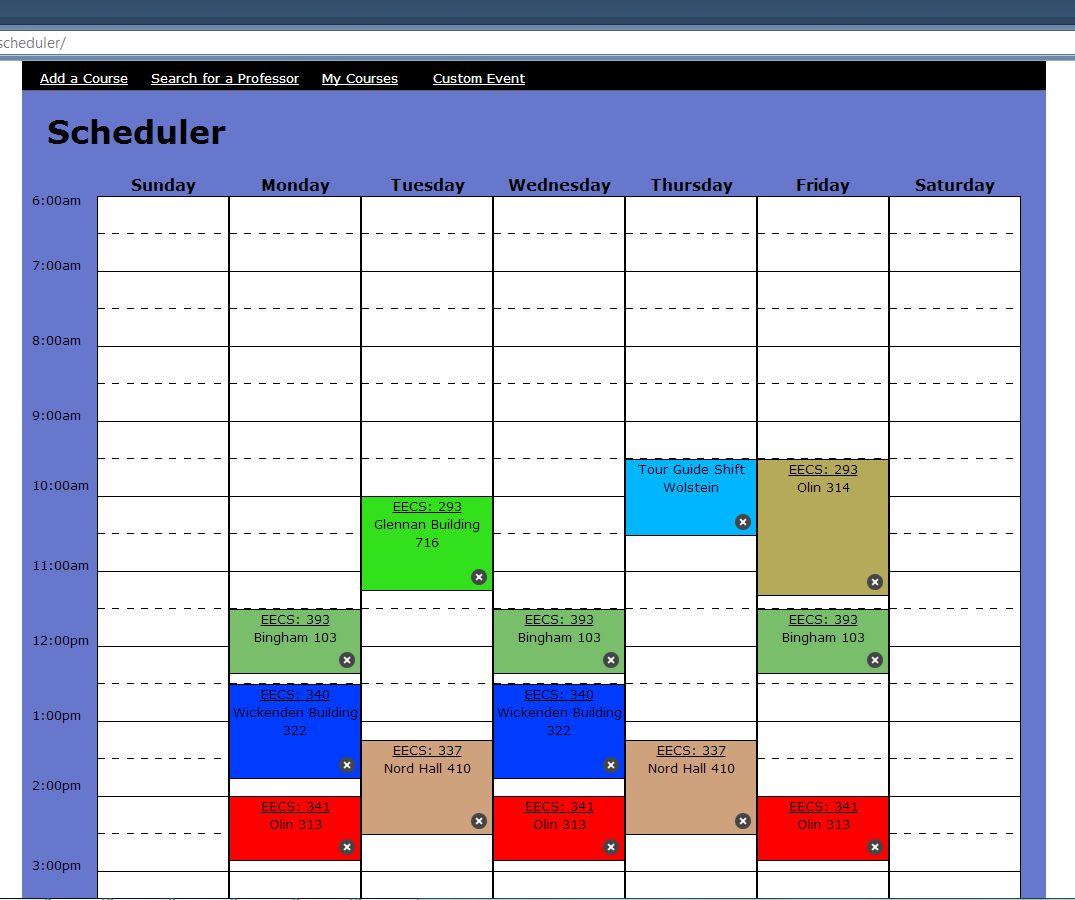
\includegraphics[width=6in]{schedule1.png}
\caption{Main page at normal zoom level with an example selection of courses and custom events}
\end{figure}
\begin{figure}
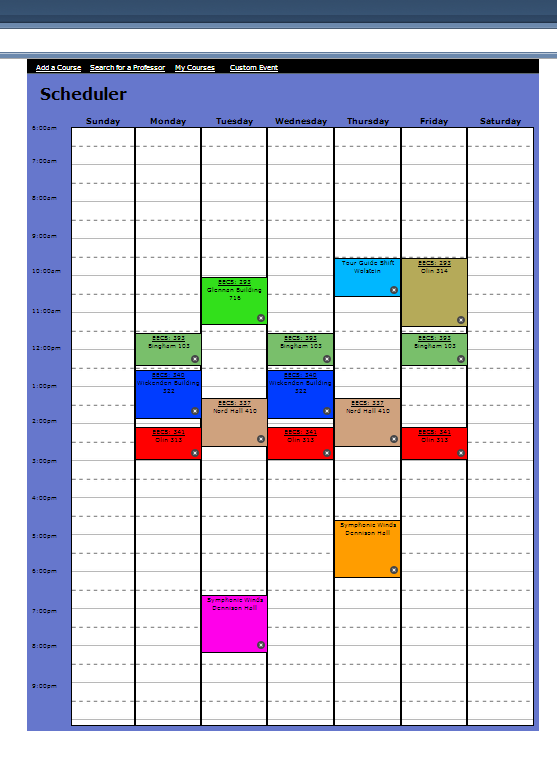
\includegraphics[width=6in]{schedule2.png}
\caption{Main page at 50\% zoom level in order to show full schedule}
\end{figure}
\FloatBarrier
\newpage
So after a user logs in and naviages \url{http://concertina.case.edu/scheduler}, the application searches urls.py for the appropriate response for that url. It see that the view for the url is 'course \_scheduler.views.schedule'. So the function schedule(request) is called in order to determine how to render the webpage. Since we have the user's id we make a query to our database via Django is order to find all of that user's events (class and custom\_events) so we can send it to the html template.\\

The final schedule seen in the figures is impemented through an HTML table. Every day of the week is a separate column in the table and just one single long row. We couldn't use sepearte rows in each column because a user's event can be at any time and span any number of time slots, and HTML table do not support any kind of span across table rows. So instead, when the schedule HTML file receives a list of events it simply creates a colored square at a location within the tabe based on that event's recur\_type (eg MWF) and start\_time. The hieght of these squares is based on the event's duration. \\

From the above screen shots you may notice that a class's title is underlined and each event has a black X button in the bottem right of its square. In designing our application we decided the two things a user would want to do from their main page was to either remove events from their schedule or see more information on a selected class. The delete button is implemented through a basic HTML form tag. The form tag is the basic HTML way to handle user input. Behind the scenes, when the user hits the click button the web page redirects to the removecourse view and passes it the user's 'request', ie that he selected to delete a certain event. The removecourse view queries the database for the enroll relationship linking the user to the specified event and deletes. Upon successful deletion, the webpage redirects back to the main schedule page. To the eyes of the user, the selected course simply disappears.\\

When the user click on a class's title, the user is taken to an information page, but that is explained more in detail below. For now, we're going to look at the second key feature for a schedule: the ability to add a class to your schedule. At the top of every page in our application there is a black navigation bar, this is built through a HTML a horizontal table HTML tag and is common to many website and was thus easy to implement. Each link brings the user to a different page of the application. The first one from the main page, "Add a Course" brings to the page show below.
\begin{figure}
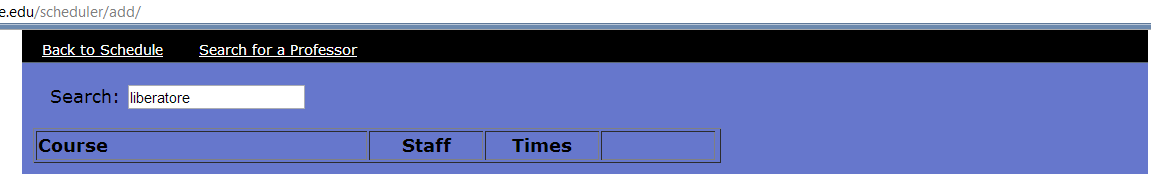
\includegraphics[width=6in]{blankAdd.png}
\caption{The add a course page as shown with no search results}
\end{figure}
\FloatBarrier
We did not encounter too many obstacles in implementing the add a course feature mostly because both the HTML and the Django queries are rather simple. The search bar is a simple form (like the delete button) with an input text field. This form calls the add view again, but this type the passed request has metadata attached to it (ie the whatever the user entered into the search box). The view queries the Instructs relationship in the database and returns a list of classes whose name, dept, and/or course number contains the search string. The HTML file then displays the classes in a table format. The figure below shows the results of a user search.
\begin{figure}
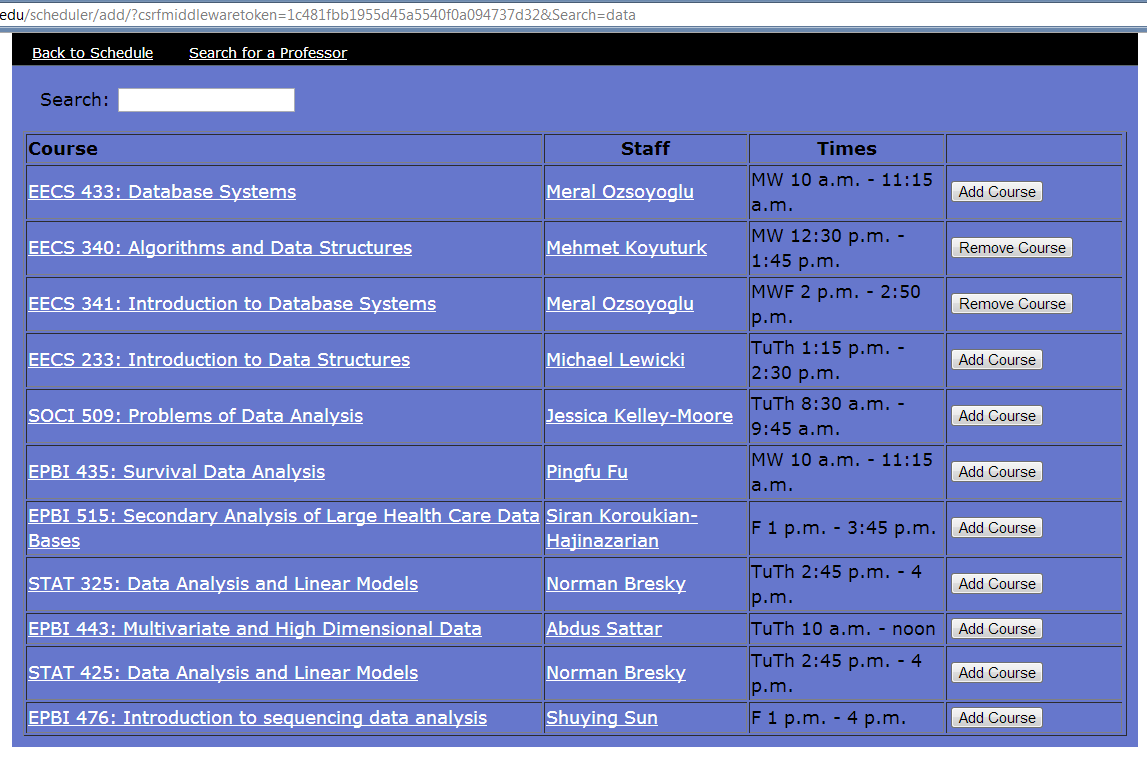
\includegraphics[width=6in]{dataResults.png}
\caption{The results returned by search for "data"}
\end{figure}
\FloatBarrier
You should see that some courses have an "Add Course" button and some have a "Remove Course" button. The courses that are already in your schedule are the ones that display "remove course." This is accomplished during the compilation of the search results, the query also checks to see if there in an Enroll relationship with the current case\_id and each returned course, and if so, that information is passed to the HTML file. The implementation for both buttons is the same as described above for the delete button from the main page.\\

Again you should see that the course title is underlined. Like on the front page, this redirects the user to a page showing information for a the selected class. In the same process, the webservice determine that the proper view is 'course \_scheduler.views.info' and sends that view the users 'request. The info view queries the database for the class with the same name as the one selected and displays a separate information table for each different meeting time for that class (or event). The results of the information page for EECS 341 are shown below.
\begin{figure}
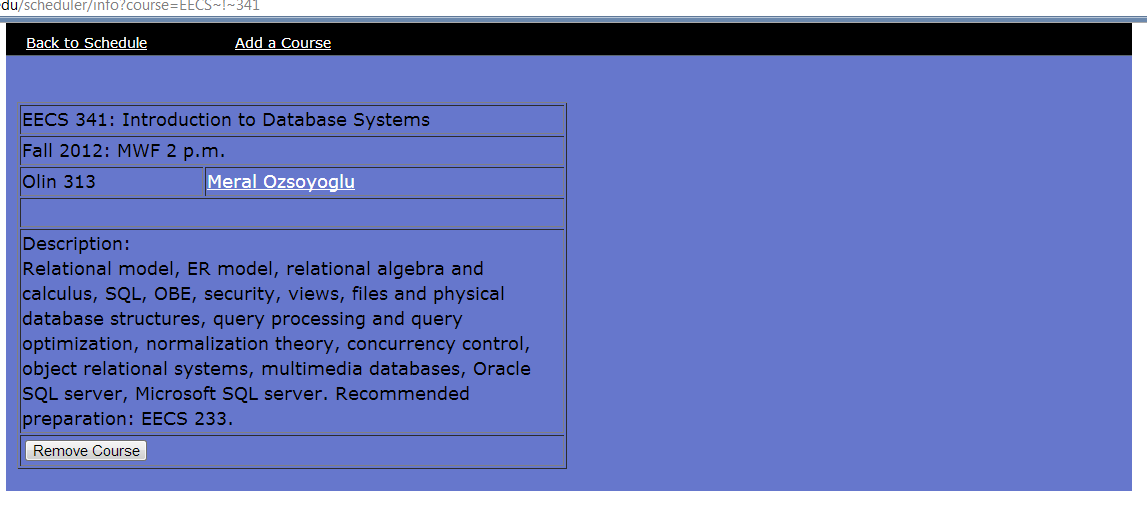
\includegraphics[width=6in]{databaseInfo.png}
\caption{The information page for EECS 341}
\end{figure}
\FloatBarrier
This page is very similar to the add page in that it displays one or more courses to the user and allows the user to selectively add or remove courses. The main difference is that the user cannot search from this page and each course has a great deal more information attached to it. By now you may be wondering exactly how the HTML accesses this information. Well, we can actually embed simple Django directly into our HTML file, allowing us to have access to the attribute of objects passed into the HTML file via the 'context' mentioned earlier. For example, the following code snipet displays a course name:\\
$\langle td \rangle${{event.meetingtime.meeting\_class.dept}} {{event.meetingtime.meeting\_class.class\_number}}: {{event.meetingtime.meeting\_class.classname}}$\langle/td \rangle$\\

Note, this is not the exact code we have, because behind the scenes the info view actually iterates through the instructs relation so that we can display an instructor for each meeting time. Also, the $\langle td \rangle$ tag is an HTML tag for whenever you want to have an entry in a table cell.\\

From here you can go back to the main schedule either through the link at the top of the page or by clicking the Add Course/Remove Course button, or you can go back to the search page by clicking "Add a Course" again, or you can go to a feature we haven't discussed, the instructor information page, by clicking on the name of the instructor, "Meral Ozsoyoglu" in the screen shot above.\\

The instructor information page, shown below, is actually the most basic page in our application. That is because, as a student scheduler, we felt that detailed instructor information was unnecessary. However, we do display an instructor's office and email address.
\begin{figure}
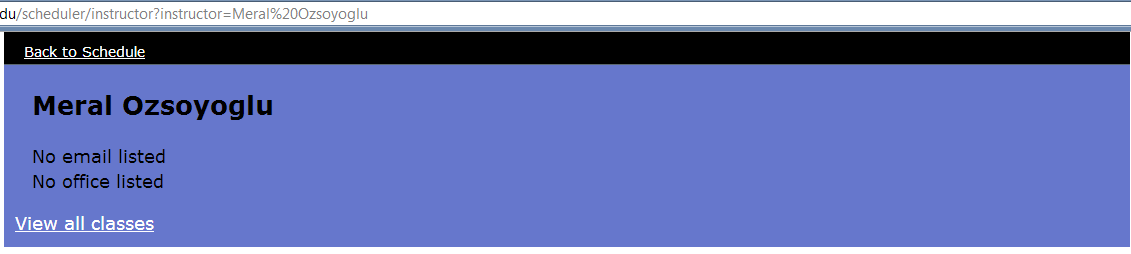
\includegraphics[width=6in]{meral.png}
\caption{The information page for Meral Ozsoyoglu}
\end{figure}
\FloatBarrier
As you can see, the office and email in this case both display as "not listed". That is because as of right now, we have not yet filled our database with an office location and email for all of the instructors present in our database. The main reason behind this lapse is that when first designing our application we beleived that this information was published by the university in the same XML document that we retrieve the course information from, but this turned out to be untrue. Thus we would now have to manually enter in all instructor information to achieve full functionality. However, because our application has the full functionality to parse an xml document and create database entries from that document, we will first ask CWRU to publish or give us access to such a list, if it exists.\\

At the bottom of the page there is a View all Courses button. This is again a HTML form button that calls the "inscourse" view, sending the view the instructor's name as a parameter. Then in that view, we query the instructs relation for all of the courses taught by the passed instructor. Then we return the resulting query set to the add HTML file discussed above. The result of hitting this button for Meral Ozsoyoglu is shown below.
\begin{figure}
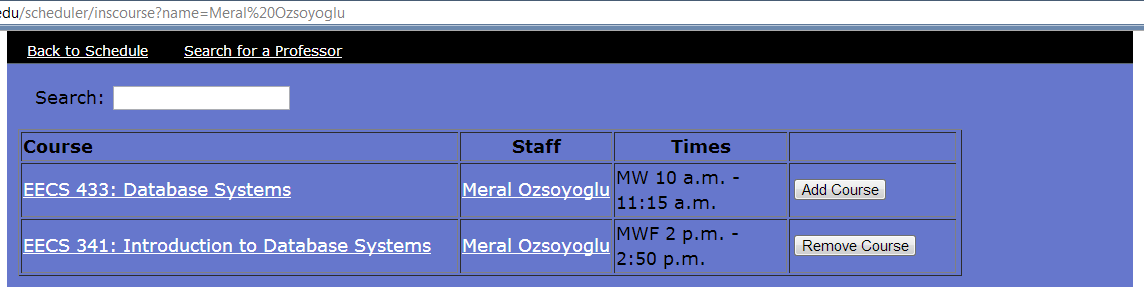
\includegraphics[width=6in]{meralCourses.png}
\caption{The courses currently taught by Meral Ozsoyoglu}
\end{figure}
\FloatBarrier

This is the familiar add page already discussed, so we're going to go ahead and return to the home page to discuss the last few features. The easiest way to do this is to hit the "Back to Schedule" button (which is available on every page except the home page). From here we'll hit the "My Courses" button. The button redirects the user to \url{http://concertina.case.edu/scheduler/mycourses}, and the urls.py file informs the application that the view to get the rendered page from is the mycourses view. This view, like the schedule views, finds all of the events for the current user, but unlike the schedule view it only queries for events with meetingtimes ie class, custom\_events (discussed below) do not have meetingtimes. Then upon a successful query, the user is redirected back to the add page, only this time the table is filled with all of the user's current classes. The result of hitting "My Courses" is shown below.
\begin{figure}
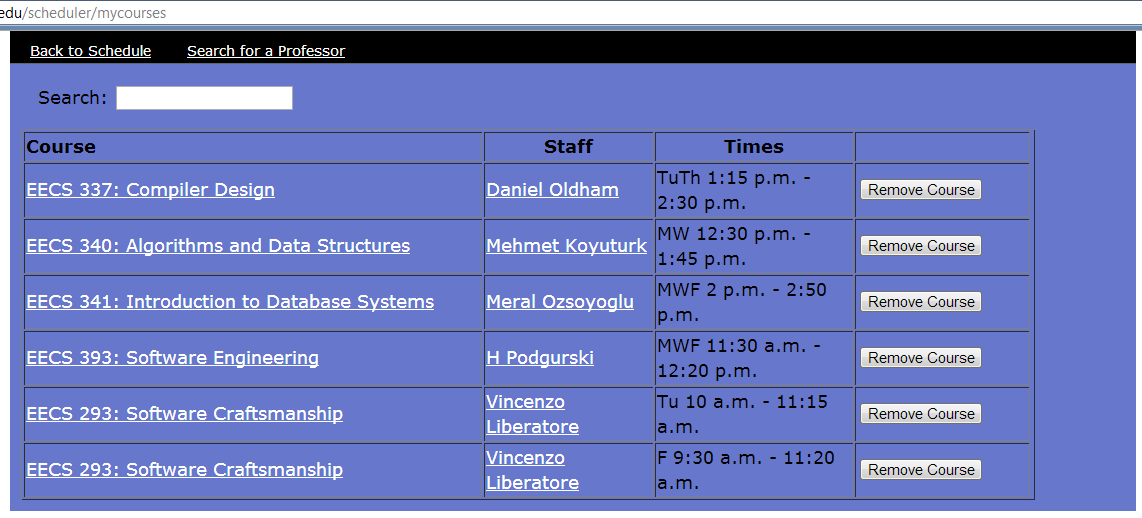
\includegraphics[width=6in]{mycourses.png}
\caption{The result of clicking the "My Courses" link}
\end{figure}
\FloatBarrier

Everything on this page functions just like the add page. That is one of the powerful parts of our application, that a lot of our HTML code can be easily reused. We could even customize this page more differently from the add page by passing in certain parameters telling the HTML file what or what not to render.\\

The final feature to discuss was the 2nd hardest implement on both the front-end and the back-end. Specifically, this feature is the idea of custom\_events. During design we decided our users' would most definitely want to be able to add their own events to their schedule. Such a feature would allow them to schedule things like extra-curricular, study-sessions, or sports practices. These events however proved troublesome when designing the database. We went through 4 or 5 different schema implementation before we settled a reasonable and effective one. This trouble stemmed from the fact that events are very similar to meetingtimes, but slightly different in key areas. For example, meetingtimes have a class associated with them that hold the class name, department, information and so forth. Thus, we couldn't have a simple custom\_event is a meetingtime relation. Nor could a meetingtime be a custom\_event because a custom\_event has attributes a meetingtime doesn't need. Finally we settled on a global event entity that both meetingtime and custom\_event could inherit from. This scheme proved difficult for our primary database developer because Django inheritance was a beast none of us had, at that point, yet touched. Fortunately Django has excellent documentation we could work with (\url{https://docs.djangoproject.com/en/dev/topics/db/models/#model-inheritance}).\\

Custom\_event proved difficult for the front-end application for entirely different reasons. First, the required a reworking of the schedule HTML code because custom\_events need to be rendered a little differently than meetingtimes. Eventually, we just decided to use a {{ if event.meetingtime }} embedded Django block in our HTML to check to see whether the event we were currently examining was a class (meetingtime) or not. Second, the creation page for an event, shown below, was a much more complex use of HTML form tags than we had used previously. One of our developers was again saved by Django's documentation as it has good coverage on Django forms and how they interact with HTML forms (\url{https://docs.djangoproject.com/en/dev/topics/forms/?from=olddocs}). They work, in short, by binding each input field in the HTML form to corresponding member attribute of a custom Django form class (see EventForm in views.py). Then when a user submits the form (by hitting the submit data), the form class checks the validity of all the entered data. If any of the data is invalid the submission is denied and an error message is displayed to the user. Else the form is sent as part of a 'request' to the proper 'view', which in this case is the "customevent" view. This view parses all of the input data and creates a new instance of a custom\_event with the corresponding attribute fields and enters it in the database. Then it grabs the current user and enters the two into an 'enroll' relation. Finally, the user is returned to the main page.
\begin{figure}
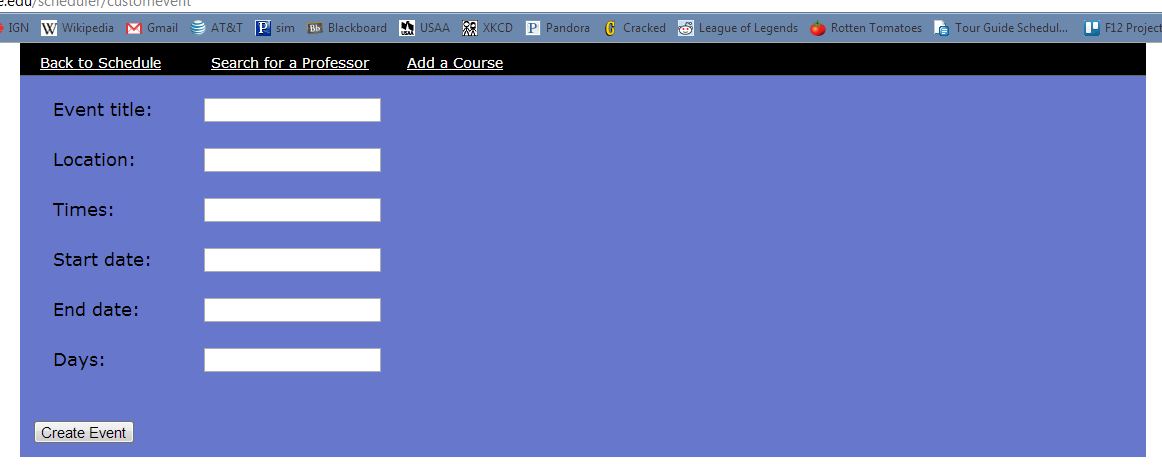
\includegraphics[width=6in]{emptyEvent.png}
\caption{The form to create an empty event}
\end{figure}
\FloatBarrier

When checking the validity of the form data, the form class calls to custom made validation methods. Both uses Python regular expressions to ensure the validty of certain fields. For example, the "days" field can only be made up for the following strings: Su M Tu W Th F Sa . Below is a figure showing some of the possible error messages.
\begin{figure}
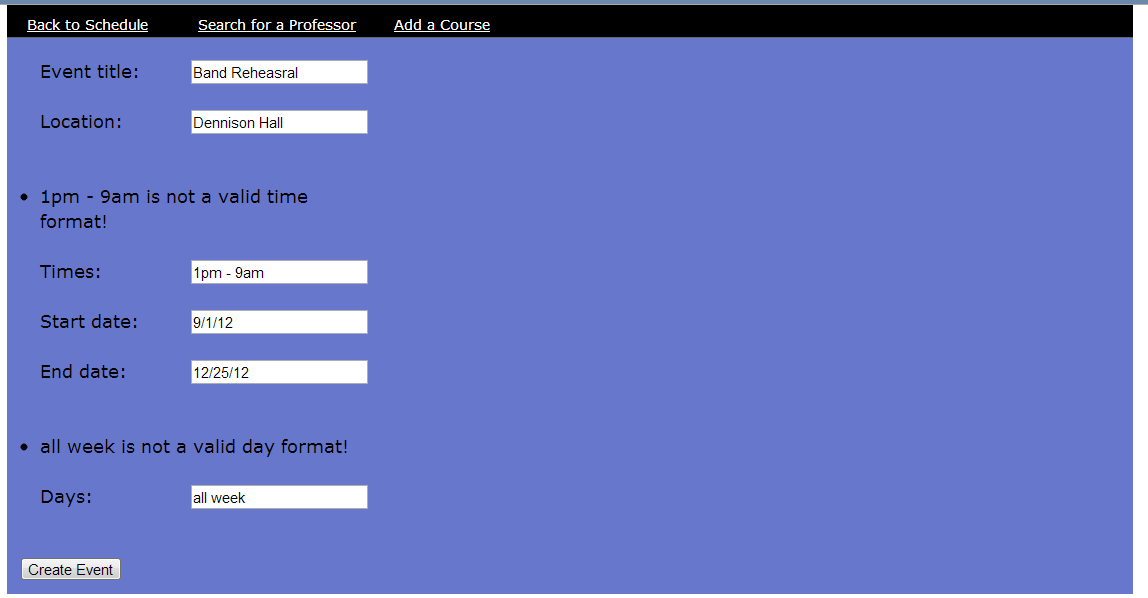
\includegraphics[width=6in]{eventErr.png}
\caption{Example of invalid custom\_event data}
\end{figure}
\FloatBarrier

That essentially covers the bare-bones of how our application implementation works. Django and HTML 5 provided a flexible and powerful way to manipulate databases, display dynamic information to the user, and respond appropriately to user input.
\appendix
\section{Appendix 1. Installation Manual}
\subsection{Installing Django and MySQL}
First, install Ubuntu or an Ubuntu-derivative.  Then execute 'apt-get install python-django mysql-server python-mysqld'.  Move the server code into a directory and set it to be on \$PYTHONPATH.  Then set the \$DJANGO\_SETTINGS\_MODULE to be the python import name of settings.py.

Log in to MySQL as the root user and run the following commands:

\begin{verbatim}
CREATE DATABASE course_scheduler;
GRANT ALL ON course_scheduler.* TO djangouser IDENTIFIED BY 'EECS341F12';
\end{verbatim}

Run 'python manage.py syncdb' and 'python manage.py reset course\_scheduler', answering yes to the prompt.

Run 'python fill\_db.py soc.xml', replacing soc.xml with the name of the soc file.

\subsection{Deployment to an Apache Server}
In order to run our application, we will be using Apache. On Ubuntu or an Ubuntu-derivative, execute 'apt-get install apache2 libapache2-mod-wsgi'. This will set up the Apache server with the mod-wsgi interface. Next, configure an Apache site in /etc/apache2/sites-available and /etc/apache2/sites-enabled. Ours is included here, and it contains elements of our directory structure which can be changed if desired.
\verbatiminput{scheduler-apache-conf.txt}
The important components of this file are as follows (more details can be found in the apache man pages)
\begin{itemize}
\item ServerName
\subitem The Fully Qualified Domain Name of the server.
\item ServerAlias
\subitem Another location at which the server can be found.
\item ServerAdmin
\subitem The email address which will be displayed upon users encountering a server error.
\item DocumentRoot
\subitem The main directory for the html files accessible by this server.
\item ErrorLog
\subitem The location to which the server's error log should be written.
\item CustomLog
\subitem The location to which all non-errors should be written
\item WSGIScriptAlias
\subitem The location at which the Python WSGI script can be located.
\item Aliases
\subitem Locations of various resources and resource folders that browsers will want.
\end{itemize}
\section{Appendix 2. User's Manual}
\subsection{Starting Case Scheduler}
To access the Case Western Reserve University scheduler you must be either  a student or faculty member at the University. Specifically, you must have a "Case ID" in order to login through Case's Single Sign-On service.\\

So, to start using the scheduler, go to \underline{http:$\\$concertina.case.edu/scheduler} and, when prompted, login with your Case ID and password. This will bring you to Case Scheduler's home page and your schedule! So anytime you actually want to view your schedule just go to \underline{http:$\\$concertina.case.edu/scheduler}\\

\subsection{Adding Courses}
As a student or professor, one of the most common events on your schedule will be classes. To add a course find the underlined "Add a Course" link at the top of the page and click.\\

You should be brought to a page with blank "Search" bar and an empty table. To search for a class enter your search criteria into the search box. The search feature currently supports search by department, course name, and/or course number.\\

So let's say you want to add "Introduction to Database Systems" to your schedule. You could try searching for "intro" or "introduction", but that would return of introduction courses at CWRU! Instead let's search for "database". Two classes should be returned: "EECS 433: Database Systems" and "EECS 341: Introduction to Database Systems".\\

You should see that the table of search results we just created displays some basic information about the courses. It displays the professor, "Meral Ozsoyoglu" in this case, the "times" for the course, and a button that adds the selected course to your schedule. As a note on the time fields, this web service uses the following convention: Sunday = Su, Monday=M, Tuesday=Tu, Wednesday=W, Thursday=Th, Friday=F, and Saturday=Sa. Let's go ahead and add EECS 341 to your schedule by clicking the "Add Course" button next to "EECS 341: Introduction to Database Systems".\\

\subsection{Course Information} 
Continuing from the "Adding Courses" section, you should be back on the main schedule page and you should have 1 class, "EECS 341", displayed on your schedule is some pleasant color.\\

Now we'll show you a different way to add a course to your schedule. Click the "Add a Course" link at the top of the page again. Let's search for "EECS 337". The search should return 1 result: "EECS 337: Compiler Design" taught by Daniel Oldham. Instead of adding the course directly from this page, we're going to go ahead and clicking on the name of the course.\\

You should have been brought to a course information page for "Compiler Design". You'll notice that a lot of different information is displayed for the course. Along with the name of the course, you should see the times and days for the course, the course location, the professor for the course, and a short description of the course. Finally, at the very bottom you should see an "Add Course" button. Go ahead and click that.

\subsection{Professors}
Continuing from the "Course Information" section, you should be back on the main schedules page and now have 2 classes in your schedule, "EECS 341" and "EECS 337". Now go ahead and click the "Search for a Professor" link at the top of the page.\\

You should be brought to a page with a "Search" bar and an empty table. Let's search for "Fred". Two results should be displayed: "Bernard Jim" and "Jim Shaffer". Go ahead and click on Professor Shaffer's name.\\

You should be brought to a short information page displaying the email and office for Professor Schafer. There should also be a link at the bottom of the page, "View all classes", go ahead and click it. This link will display all the classes currently taught by Professor Shaffer.\\

In this case, only 2 courses will be displayed "ANTH 331" and "ANTH 107". You may notice that we are the same type of page as the "Add a Course" page, and you'd be right! You should notice that from this page you could also click on "Jim Shaffer" and that would just take you back to your Professor Shaffer's page again. Let's go ahead and ad "ANTH 107" to our schedule by clicking the "Add Course" button.\\

\subsection{My Courses}
Continuing from the "Professors" section, you should once again be back on the main schedule page, but now have 3 classes in your schedule. Let's go ahead and click the "My Courses" link at the top of the screen.\\

You should be brought to a table displaying the list of the 3 courses currently in your schedule. You'll that it's exactly the same as an "Add a Course Page". Let's go ahead and remove "ANTH 107" from your schedule by clicking the "Remove Course" button, because who wants to take anthropology anyway? Note, that this "Remove Course" button will be available anywhere where you have seen an "Add Course" button for the classes that are already in your schedule. You should be brought back to the main schedule page and now you should see that "ANTH 107" is no longer in your schedule.\\

\subsection{Courses on the Schedule}
Continuing on from the "My Courses" section, you should have 2 courses currently in your schedule. Notice that the names of the courses are underlined, this means that they represent links. Let's go ahead and click on "EECS 337". You should be brought to the familiar course information page for EECS 337, though now it says "Remove Course" at the bottom instead of "Add Course". Go ahead and click "Remove Course", you should be brought to the main schedule page, and now EECS 337 should no longer be in the your schedule.\\

Look at the last course in your schedule, EECS 341, you should see an "X" icon in the bottom right of the colored course. Clicking this button removes the select event from your schedule, go ahead and remove EECS 341 from the schedule.

\subsection{Custom Events}
Continuing on from the "Courses on the Schedule", you will now learn how to add your own events to your schedule. Go ahead and click the "Custom Event" link at the top of the page. You should see a series of text fields that correspond to information you want to enter for your custom event. Note that all fields are mandatory.\\

"Event title" corresponds to the name of your event, and will be what is actually displayed on your schedule. The "Times" field represents the duration of your event. NOTE: your choice time must be passed in in the following format: "xx:xxAM/PM - xx:xxAM/PM" where x is a valid digit 0-9. Note that a time such as "9:00" can be entered in as such, it does not have to be "09:00". Also the end time for the interval cannot be before te start time.\\

The "Start Date" and "End Date" fields correspond to the time period during which you want your event to recur. These dates should be entered in in the dd/mm/yy format. Finally the days field corresponds to on which days your event recurs. E.G. MWF would correspond to "Monday", "Wednesday", and "Friday". Go ahead and create a custom event and add it to your schedule. On clicking "Create Event" you should be returned to the main schedule page, and you should see your event on your schedule. If you want to delete a custom event, simply click the the "x" button as you would to delete a course.\\

Congratulations, you've successfully made it through he entire basic User's Manual for the new Case Scheduler. If you have any questions, comments, or concerns, please email our dev team at stuart.long@case.edu

\end{document}
